\chapter{Rynek walutowy}

\section{Historia i rozwój rynku walutowego}
\subsection{Starożytność}
Historia rynku walutowego sięga początków międzynarodowych stosunków gospodarczych. Jego rozwój był ściśle związany ze zmianami w systemach walutowych oraz rozwojem handlu międzynarodowego. 
Pierwsze formy wymiany walut powstały już w starożytności, kiedy wzrastał handel między europejskimi śródziemnomorskimi państwami oraz krajami bliskiego wschodu i azji. 
Wymianę barterową stopniowo zastępowała wymiana monetarna, w której o wartości monety decydowała zawartość kruszca, z której została ona wykonana. 
W rozwinętych włoskich miastach powstali pierwsi pośrednicy finansowi, zajmujący się wymianą walut o różnej zawartości kruszca i różnym pochodzeniu \parencite{melvin2013}. 

W kolejnych wiekach w starożytnym Rzymie powstał rozbudowany system monetarny oparty na srebrnym denarze, który stanowił podstawową jednostkę rozliczeniową w Imperium. 
Ujednolicenie wartości monet w oparciu o srebro umożliwiło rozwój handlu międzyregionalnego, co można uznać za wczesną formę zorganizowanego systemu walutowego \parencite{melvin2013}. 

\subsection{Średniowiecze}
Po upadku Cesarstwa Rzymskiegos ograniczono handel dalekosiężny, a znaczenie wymiany walutowej zmalało, lecz już w okresie średniowiecza powrócił w nowej formie. 
W europejskich miastach rozwijały się nowe prywatne instytucje finansowe zajmujące się wymianą walut, kredytem kupieckim oraz transferem środków między państwami. 
To właśnie w tym okresie powstały pierwsze weksle, listy kredytowe i rachunki rozliczeniowe, które można uznać za pierwowzory współczesnych instrumentów finansowych \parencite{mishkin2018}.

\subsection{XX wiek}
Przez większą część XX wieku funkcjonował system oparty na stałych kursach walutowych, którego podstawą był standard złota. 
Był systemem monetarnym, w którym wartość waluty krajowej opierała się na określonej ilości złota, a państwa utrzymywały stałe kursy wymiany między sobą. 
System ten zapewniał wysoką stabilność kursów walutowych, lecz ograniczał elastyczność polityki monetarnej, co ostatecznie doprowadziło do jego upadku w XX wieku \parencite{mishkin2018}.

Po II wojnie światowej przyjęto system z Bretton Woods, w ramach którego kursy walut powiązano z dolarem amerykańskim, a ten z kolei był wymienialny na złoto. 
System ten zapewniał względną stabilność międzynarodowych rozliczeń, jednak jego sztywność doprowadziła do narastających napięć gospodarczych \parencite{mishkin2018}. 

W 1971 roku prezydent Stanów Zjednoczonych Richard Nixon ogłosił zawieszenie wymienialności dolara na złoto, co w praktyce oznaczało koniec systemu z Bretton Woods. 
W kolejnych latach kraje zaczęły wprowadzać płynne kursy walutowe, co zapoczątkowało powstanie nowoczesnego rynku Forex w formie zdecentralizowanej sieci wymiany walut międzybankowych \parencite{hull2018}. 
Jak wskazuje Hull, upadek systemu stałych kursów był punktem zwrotnym w historii współczesnych finansów międzynarodowych, od tego momentu kursy walut zaczęły kształtować się w sposób rynkowy,
w oparciu o mechanizm popytu i podaży. 

Lata 80. i 90. XX wieku przyniosły gwałtowny rozwój rynku walutowego w związku z liberalizacją przepływów kapitałowych, rozwojem telekomunikacji oraz informatyzacji. 
W tym okresie pojawiły się pierwsze elektroniczne platformy transakcyjne, które zastąpiły tradycyjny rynek międzybankowy oparty na kontaktach telefonicznych. 
Z czasem rynek Forex zaczął przyciągać także inwestorów instytucjonalnych i detalicznych, co uczyniło go najbardziej płynnym rynkiem finansowym na świecie \parencite{zukowski2014}. 
Jak podaje Bank for International Settlements, dzienny obrót na globalnym rynku Forex wzrósł z około 590 miliardów dolarów amerykańskich w 1989 roku do ponad 7{,}5 biliona dolarów w 2022 roku \parencite{bis2022}.
Dane te obrazują skalę dynamicznego rozwoju tego rynku oraz jego rosnące znaczenie w światowym systemie finansowym. 

Na tle tych globalnych przemian również w Polsce zaczęły kształtować się warunki sprzyjające rozwojowi rynku walutowego. 
Początki rodzimego rynku Forex sięgają lat 90. XX wieku, kiedy to w wyniku otwarcia gospodarki i liberalizacji obrotu dewizowego możliwe stało się prowadzenie transakcji walutowych na szerszą skalę.
Początkowo uczestniczyły w nim głównie banki komercyjne, jednak wraz z postępem technologicznym i upowszechnieniem internetowych platform transakcyjnych rynek ten stał się dostępny również dla inwestorów indywidualnych.
Jak zauważają Furman i Hańczyk \parencite{furman2016}, istotną rolę w rozwoju krajowego segmentu rynku Forex odegrały zmiany regulacyjne oraz napływ zagranicznych brokerów internetowych.

Obecnie rynek Forex stanowi w pełni zdecentralizowany i globalny system wymiany walut, w którym uczestniczą zarówno banki centralne i komercyjne, jak i fundusze inwestycyjne, korporacje oraz inwestorzy detaliczni.
Jego ewolucja — od tradycyjnych kontaktów telefonicznych po nowoczesne platformy elektroniczne — odzwierciedla szersze procesy integracji rynków finansowych, cyfryzacji oraz globalizacji gospodarki światowej.

\section{Charakterystyka rynku Forex}

\subsection{Struktura i organizacja}

Rynek walutowy (Foreign Exchange Market, w skrócie Forex) jest rynkiem pozagiełdowym, co oznacza, że transakcje nie są zawierane na jednej scentralizowanej giełdzie,
lecz realizowane bezpośrednio pomiędzy uczestnikami za pośrednictwem sieci banków, brokerów oraz elektronicznych platform handlowych \parencite{bis2022}. 
Zdecentralizowany charakter rynku sprawia, że kursy walut kształtują się w sposób płynny w wyniku interakcji podaży i popytu w różnych centrach finansowych na całym świecie,
a nie w jednym punkcie notowań, jak ma to miejsce na tradycyjnych giełdach papierów wartościowych. 
Taka struktura sprzyja wysokiej elastyczności handlu, globalnemu zasięgowi oraz stałemu dostępowi do rynku niemal przez całą dobę.

Uczestnikami rynku Forex są różnorodne podmioty, które można podzielić na kilka głównych grup. 
Najważniejszą rolę odgrywają banki komercyjne i inwestycyjne, które stanowią głównych dostawców płynności, realizując transakcje zarówno między sobą, jak i ze swoimi klientami instytucjonalnymi. 
Istotnym uczestnikiem są również banki centralne, które wchodzą na rynek w celu stabilizacji kursów walutowych lub realizacji polityki monetarnej. 
Kolejną grupę stanowią korporacje międzynarodowe, dokonujące transakcji walutowych w związku z handlem zagranicznym, inwestycjami zagranicznymi czy zabezpieczaniem ryzyka kursowego. 
Ważną rolę pełnią także fundusze inwestycyjne oraz hedgingowe, które wykorzystują rynek do celów spekulacyjnych, arbitrażowych i zabezpieczających. 
W ostatnich latach coraz większe znaczenie zyskują również inwestorzy indywidualni, którzy dzięki rozwojowi technologii i internetowych platform tradingowych uzyskali bezpośredni dostęp do rynku \parencite{madura2018}. 
Motywacje uczestników rynku można zatem sprowadzić do trzech głównych kategorii: transakcyjnych, związanych z wymianą walut w działalności gospodarczej; 
zabezpieczających, czyli redukcji ryzyka kursowego; oraz spekulacyjnych, nastawionych na osiągnięcie zysku z krótkoterminowych zmian kursów.

Rynek Forex funkcjonuje nieprzerwanie przez 24 godziny na dobę, pięć dni w tygodniu. 
Handel rozpoczyna się w poniedziałek rano w Sydney, następnie przenosi się do Tokio, Londynu i Nowego Jorku, po czym cykl powtarza się aż do piątkowego wieczoru czasu nowojorskiego.
Dzięki temu uczestnicy rynku mają możliwość handlu w różnych strefach czasowych, co czyni Forex rynkiem o wyjątkowej ciągłości działania. 
Największa aktywność handlowa obserwowana jest w okresach nakładania się sesji europejskiej i amerykańskiej, kiedy płynność oraz zmienność są najwyższe \parencite{bis2022},
co ma miejsce zazwyczaj między godziną 13:00 a 17:00 czasu polskiego zimą (lub 14:00–18:00 latem), gdy jednocześnie aktywne są rynki w Londynie i Nowym Jorku.

Rynek Forex charakteryzuje się bardzo wysoką płynnością, co oznacza możliwość szybkiego zawierania transakcji o dużych wolumenach bez znaczącego wpływu na cenę rynkową. 
Według danych Banku Rozrachunków Międzynarodowych (BIS) z 2022 roku dzienny obrót na rynku walutowym przekraczał 7,5 biliona dolarów amerykańskich \parencite{bis2022}.
Tak ogromna skala obrotu sprawia, że Forex jest największym i najbardziej płynnym rynkiem finansowym na świecie.
Należy jednak zaznaczyć, że płynność nie jest stała w czasie. Zmienia się w zależności od pory dnia, aktywności poszczególnych centrów finansowych oraz publikacji istotnych danych makroekonomicznych,
które wpływają na zmienność kursów.

\subsection{Mechanizm działania rynku}

Transakcje na rynku Forex odbywają się zawsze w formie par walutowych, gdzie jedna waluta pełni funkcję waluty bazowej, a druga waluty kwotowanej. 
Kurs walutowy określa, ile jednostek waluty kwotowanej należy zapłacić za jedną jednostkę waluty bazowej. 
Przykładowo, kurs EUR/USD = 1,10 oznacza, że za jedno euro należy zapłacić 1,10 dolara amerykańskiego. 
Notowania walutowe są nieustannie aktualizowane w czasie rzeczywistym, a ich wartość kształtowana jest przez relację popytu i podaży na dane waluty na rynku globalnym \parencite{hull2018}. 
Najbardziej płynne i najczęściej handlowane pary walutowe określa się mianem „major pairs” i należą do nich: EUR/USD (euro do dolara amerykańskiego),
USD/JPY (dolar amerykański do jena japońskiego), GBP/USD (funt szterling do dolara amerykańskiego), USD/CHF (dolar amerykański do franka szwajcarskiego), 
AUD/USD (dolar australijski do dolara amerykańskiego) oraz USD/CAD (dolar amerykański do dolara kanadyjskiego). 
Pary te generują ponad 70\% całkowitego obrotu na rynku Forex, z czego wynika charakterystyczna dla nich wysoka płynność. 
Pary te charakteryzują się również dużym znaczeniem gospodarek emitujących dane waluty oraz szerokiej dostępności danych rynkowych \parencite{bis2022}. 
Pozostałe pary, określane mianem „minor pairs” lub „crosses”, obejmują waluty głównych gospodarek, ale bez udziału dolara amerykańskiego (np. EUR/GBP czy EUR/JPY), 
natomiast pary „egzotyczne” (\textit{exotic pairs}) łączą waluty gospodarek rozwiniętych z walutami krajów wschodzących, charakteryzując się niższą płynnością i wyższą zmiennością.

Transakcje walutowe mogą przybierać różne formy w zależności od horyzontu czasowego oraz celu ekonomicznego. 
Podstawowym rodzajem jest transakcja \textit{spot}, czyli natychmiastowa wymiana walut z rozliczeniem zazwyczaj w ciągu dwóch dni roboczych. 
Kolejnym typem są transakcje terminowe, do których należą kontrakty \textit{forward}, \textit{swap} oraz instrumenty pochodne, takie jak \textit{futures} i \textit{opcje walutowe}. 
Transakcje typu forward polegają na uzgodnieniu kursu wymiany w dniu zawarcia kontraktu, przy jednoczesnym ustaleniu przyszłego terminu jego realizacji, 
co pozwala uczestnikom zabezpieczyć się przed ryzykiem kursowym. Transakcje swapowe stanowią kombinację operacji kupna i sprzedaży tej samej waluty z różnymi datami rozliczenia, 
natomiast kontrakty futures i opcje walutowe są przedmiotem obrotu na rynkach regulowanych lub w ramach platform elektronicznych i służą zarówno do zabezpieczania pozycji, 
jak i do spekulacji \parencite{hull2018}.

Rynek Forex funkcjonuje w modelu dwustronnych kwotowań, w którym każdy instrument finansowy posiada dwa kursy: kurs kupna (\textit{bid}) i kurs sprzedaży (\textit{ask}). 
Różnica pomiędzy nimi, określana mianem \textit{spreadu}, stanowi podstawowy koszt transakcyjny oraz źródło zysku dla dostawców płynności, takich jak banki i brokerzy. 
Wysokość spreadu zależy od płynności danej pary walutowej, wolumenu transakcji oraz aktualnej zmienności rynkowej. 
Na najbardziej płynnych parach, takich jak EUR/USD czy USD/JPY, spread może wynosić zaledwie kilka jednostek pipsa, natomiast na parach egzotycznych jest zdecydowanie większy \parencite{bis2022}.

Istotną cechą handlu na rynku Forex jest wykorzystanie dźwigni finansowej (\textit{leverage}), która umożliwia inwestorom kontrolowanie pozycji o wartości wielokrotnie przewyższającej posiadany kapitał. 
Dźwignia pozwala na zwiększenie potencjalnych zysków, ale jednocześnie wiąże się ze znacznym ryzykiem poniesienia strat przekraczających depozyt zabezpieczający. 
Wysokość dostępnej dźwigni zależy od rodzaju uczestnika rynku, regulacji krajowych oraz polityki danego brokera. 
W przypadku inwestorów detalicznych w Unii Europejskiej, zgodnie z wytycznymi ESMA, maksymalna dźwignia dla głównych par walutowych wynosi 1:30, 
natomiast dla inwestorów profesjonalnych może być znacznie wyższa \parencite{esma2018}.

W praktyce handlu na rynku Forex istotną rolę odgrywa także wielkość jednostek transakcyjnych. 
Standardową jednostką obrotu jest tzw. \textit{lot}, odpowiadający 100 000 jednostkom waluty bazowej. 
Wraz z rozwojem rynku detalicznego wprowadzono mniejsze jednostki: \textit{mini lot} (10 000 jednostek) oraz \textit{mikro lot} (1 000 jednostek), które umożliwiły uczestnictwo inwestorom indywidualnym dysponującym mniejszym kapitałem \parencite{madura2018}. 
Handel przy użyciu mniejszych jednostek wiąże się jednak z relatywnie niższą wartością pozycji, przez co potencjalne zyski mogą być częściowo pochłonięte przez koszty transakcyjne.

W kontekście wykorzystania dźwigni finansowej szczególnie istotny jest wymóg utrzymywania tzw. depozytu zabezpieczającego (\textit{margin}), który stanowi część wartości otwartej pozycji. 
W przypadku niekorzystnych zmian kursu i spadku wartości depozytu poniżej wymaganego poziomu broker ma prawo do wezwania inwestora do jego uzupełnienia (\textit{margin call}) 
lub zamknięcia pozycji w celu ograniczenia dalszych strat. Oprócz spreadu inwestorzy ponoszą również inne koszty, takie jak prowizje od transakcji oraz tzw. \textit{swap}, 
czyli opłatę za utrzymanie otwartej pozycji przez noc. Swap odzwierciedla różnicę w stopach procentowych pomiędzy dwiema walutami tworzącymi parę i może mieć charakter dodatni lub ujemny, 
w zależności od kierunku transakcji i polityki monetarnej danego kraju \parencite{esma2018}.

Na kształtowanie kursów walutowych wpływa wiele czynników o charakterze zarówno ekonomicznym, jak i psychologicznym. 
Do najważniejszych należą różnice w poziomie stóp procentowych pomiędzy krajami, dane makroekonomiczne (takie jak inflacja, produkt krajowy brutto czy bilans handlowy), 
polityka monetarna banków centralnych oraz sytuacja geopolityczna. Dodatkowo, rosnący udział handlu algorytmicznego i automatyzacja procesów decyzyjnych sprawiają, 
że zmienność kursów może w krótkim okresie reagować na mikrostrukturalne czynniki rynkowe, takie jak wolumen obrotu czy publikacje danych w czasie rzeczywistym \parencite{chaboud2023}.

W przypadku inwestorów indywidualnych transakcje na rynku Forex realizowane są za pośrednictwem brokerów detalicznych, którzy udostępniają elektroniczne platformy transakcyjne, 
takie jak MetaTrader 4, MetaTrader 5 czy cTrader. Platformy te umożliwiają składanie zleceń kupna i sprzedaży w czasie rzeczywistym, monitorowanie notowań rynkowych, 
analizę techniczną oraz automatyzację handlu za pomocą tzw. ekspertów (EA – \textit{Expert Advisors}).

Inwestor może wybierać pomiędzy różnymi rodzajami zleceń, w tym zleceniami rynkowymi (\textit{market orders}), realizowanymi po bieżącej cenie rynkowej, oraz zleceniami oczekującymi (\textit{pending orders}), 
które aktywują się po osiągnięciu określonego poziomu ceny. Dodatkowo dostępne są mechanizmy zarządzania ryzykiem, takie jak zlecenia obronne \textit{stop loss} oraz zlecenia realizacji zysku \textit{take profit}, 
które automatycznie zamykają pozycję po osiągnięciu wyznaczonych progów.

Brokerzy mogą działać w różnych modelach rynkowych, m.in. \textit{Dealing Desk} (market maker), gdzie broker jest stroną transakcji i sam kształtuje kwotowania, 
lub w modelach \textit{STP} (Straight Through Processing) i \textit{ECN} (Electronic Communication Network), w których zlecenia klientów przekazywane są bezpośrednio na rynek międzybankowy. 
Model ECN charakteryzuje się zazwyczaj węższymi spreadami i większą transparentnością, lecz często wiąże się z dodatkowymi prowizjami transakcyjnymi.

Proces handlu u inwestorów detalicznych jest w pełni zautomatyzowany, a rozliczenia odbywają się w czasie rzeczywistym. 
Inwestor wpłaca środki w walucie bazowej rachunku (np. USD lub PLN), które stanowią depozyt zabezpieczający (\textit{margin}) i umożliwiają otwieranie pozycji z wykorzystaniem dźwigni finansowej. 
Całość procesu, od składania zleceń po rozliczenie, odbywa się elektronicznie bez fizycznej wymiany walut.

\subsection{Czynniki kształtujące kursy walutowe}

Kursy walutowe kształtują się w wyniku złożonych interakcji między wieloma czynnikami ekonomicznymi, politycznymi i rynkowymi. 
Jednym z najważniejszych czynników jest poziom stóp procentowych w poszczególnych krajach. 
Wyższe stopy procentowe przyciągają inwestorów zagranicznych, poszukujących wyższej stopy zwrotu, co prowadzi do zwiększonego popytu na walutę danego kraju i jej aprecjacji. 
Z kolei obniżki stóp procentowych często skutkują osłabieniem waluty, ponieważ zmniejszają atrakcyjność inwestycji denominowanych w tej walucie \parencite{madura2018}.

Istotne znaczenie mają również dane makroekonomiczne, takie jak tempo wzrostu gospodarczego (PKB), inflacja, poziom bezrobocia czy bilans handlowy. 
Pozytywne wyniki gospodarcze wzmacniają zaufanie inwestorów i przyczyniają się do wzrostu wartości waluty, natomiast słabe dane mogą prowadzić do jej deprecjacji. 
Na przykład wzrost inflacji powyżej oczekiwań rynkowych może sugerować konieczność zacieśnienia polityki monetarnej przez bank centralny, co często skutkuje umocnieniem waluty w krótkim okresie.

Znaczącym czynnikiem wpływającym na notowania walut są decyzje i komunikaty banków centralnych, które określają kierunek polityki pieniężnej. 
Oczekiwania dotyczące przyszłych zmian stóp procentowych, programów skupu aktywów (QE) czy interwencji walutowych mają natychmiastowy wpływ na rynki. 
Przykładowo, jastrzębie wypowiedzi przedstawicieli Rezerwy Federalnej (Fed) zazwyczaj prowadzą do umocnienia dolara amerykańskiego.

Nie bez znaczenia pozostają również czynniki geopolityczne i psychologiczne. 
Konflikty zbrojne, napięcia handlowe, kryzysy polityczne czy zmiany rządów mogą powodować gwałtowne przepływy kapitału w kierunku tzw. „bezpiecznych przystani”, 
takich jak dolar amerykański, frank szwajcarski czy złoto. 
Współcześnie dużą rolę odgrywają także czynniki behawioralne i nastroje inwestorów, które potrafią wzmacniać trendy rynkowe niezależnie od fundamentów ekonomicznych.

W ostatnich latach coraz większe znaczenie w kształtowaniu kursów walut zyskał handel algorytmiczny oraz automatyzacja procesów inwestycyjnych. 
Systemy oparte na sztucznej inteligencji i analizie danych w czasie rzeczywistym reagują błyskawicznie na publikacje makroekonomiczne i zmiany cen, 
co zwiększa krótkoterminową zmienność, zwłaszcza na najpłynniejszych parach walutowych \parencite{chaboud2023}.

\subsection{Statystyki i znaczenie rynku Forex}

Rynek walutowy pozostaje największym segmentem światowych finansów pod względem wartości obrotu. 
Według danych Banku Rozrachunków Międzynarodowych (BIS) z 2022 roku, dzienny obrót na globalnym rynku walutowym przekraczał 7,5 biliona dolarów amerykańskich,
z czego około 88\% wszystkich transakcji obejmowało dolara amerykańskiego \parencite{bis2022}. 
Oznacza to, że niemal każda operacja na rynku walutowym wiąże się z udziałem USD jako waluty bazowej lub kwotowanej, co czyni go bezsprzecznie najważniejszą walutą międzynarodową.
Na drugim miejscu znajduje się euro, które uczestniczy w 32\% transakcji, natomiast jen japoński w około 17\%. 
Udział pozostałych walut, w tym chińskiego juana (CNY) oraz funta szterlinga (GBP), systematycznie rośnie, co odzwierciedla przesuwanie się centrum ciężkości światowego handlu w kierunku Azji.

Na Rys.~\ref{fig:bis_turnover} przedstawiono średni dzienny obrót według rodzaju instrumentu. 
Widać wyraźnie, że największy udział mają transakcje typu \textit{FX swap}, które stanowią ponad połowę całkowitego obrotu, natomiast transakcje \textit{spot} odpowiadają za około jedną trzecią. 
Struktura ta jest typowa dla rynku międzybankowego, gdzie większość uczestników dokonuje transakcji o charakterze zabezpieczającym lub służących zarządzaniu płynnością, a nie spekulacji. 
Warto zauważyć, że mimo dominacji segmentu \textit{swap}, znaczenie transakcji natychmiastowych utrzymuje się na wysokim poziomie, 
co dowodzi stałego zapotrzebowania na bieżącą wymianę walut w globalnym handlu i finansach.

\begin{figure}[h!]
  \centering
  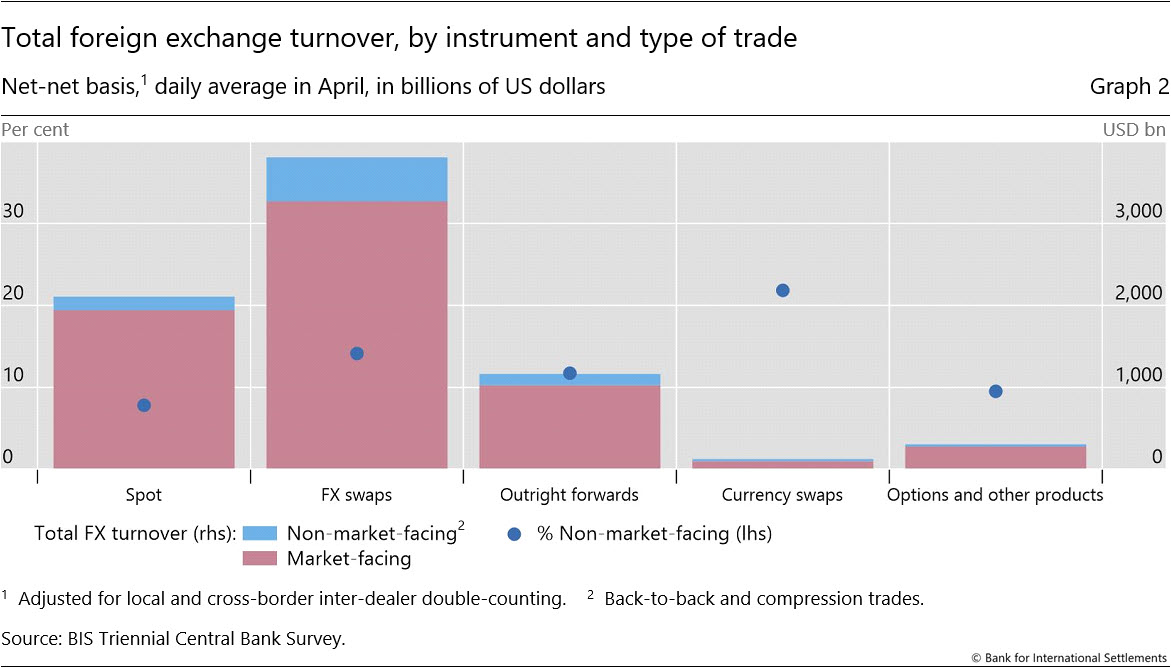
\includegraphics[width=0.85\textwidth]{plots/bis_fx_turnover_by_instrument_2022.jpg}
  \caption{Średni dzienny obrót na globalnym rynku walutowym według instrumentu w 2022 roku (w bln USD). Źródło: BIS (2022), \textit{Triennial Central Bank Survey}.}
  \label{fig:bis_turnover}
\end{figure}

Na poziomie walutowym (Rys.~\ref{fig:bis_pairs}) dominującą rolę odgrywa dolar amerykański (USD), który uczestniczy w 88\% wszystkich transakcji, 
a także euro (32\%) oraz jen japoński (17\%). Wśród najczęściej handlowanych par walutowych największy udział mają EUR/USD, USD/JPY oraz GBP/USD, 
co odzwierciedla dominację głównych gospodarek światowych w międzynarodowych przepływach kapitału. 
Warto zwrócić uwagę, że udział chińskiego juana (CNY) w obrotach Forex wzrósł w 2022 roku do około 7\%, co stanowi najwyższy poziom w historii i potwierdza rosnące znaczenie Chin w systemie finansowym. 
Mimo to udział walut rynków wschodzących wciąż pozostaje ograniczony z uwagi na niższą płynność i większe ryzyko regulacyjne.

\begin{figure}[h!]
  \centering
  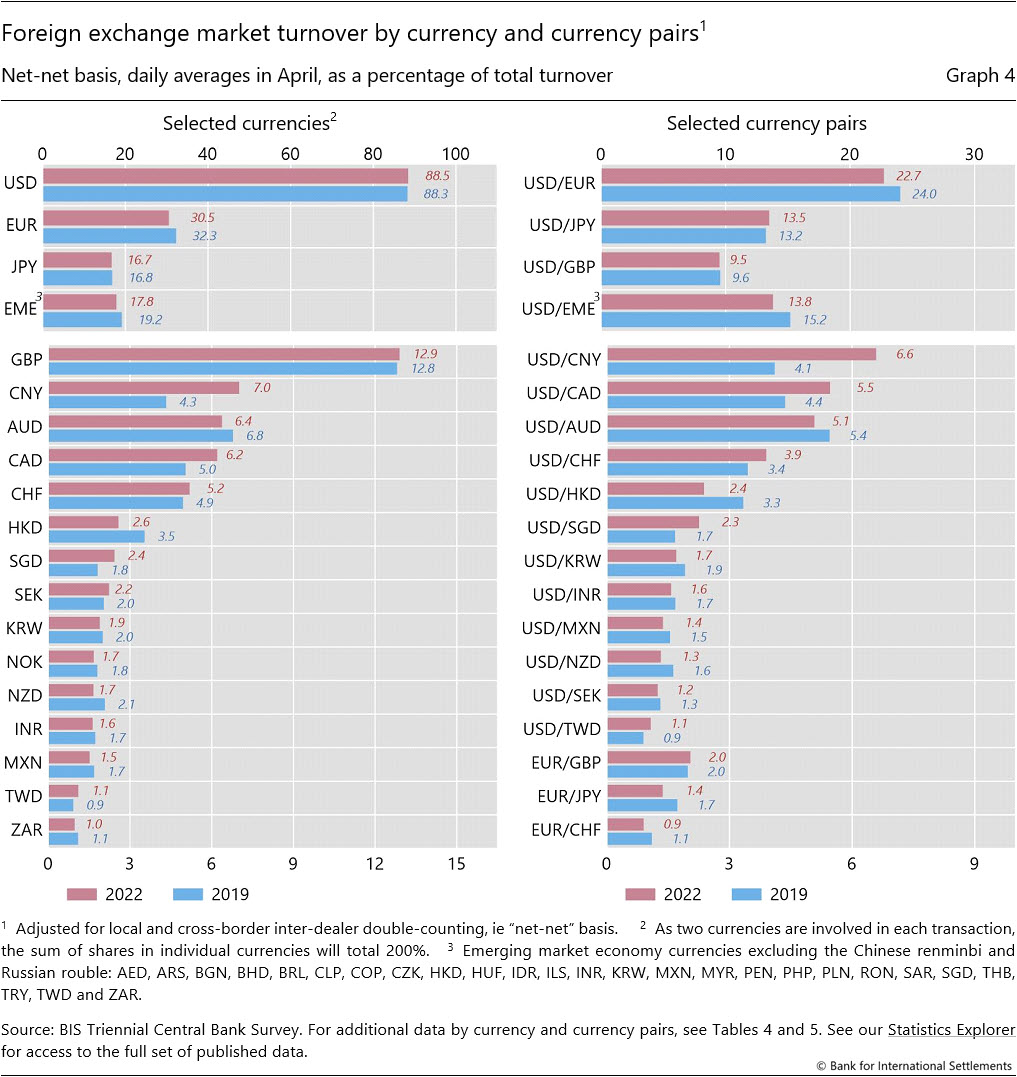
\includegraphics[width=0.9\textwidth]{plots/bis_fx_turnover_pairs_2022.jpg}
  \caption{Udział głównych walut i par walutowych w globalnym obrocie na rynku walutowym w 2022 roku (w \%). Źródło: BIS (2022), \textit{Triennial Central Bank Survey}.}
  \label{fig:bis_pairs}
\end{figure}

W kontekście Polski, zgodnie z wynikami badania Narodowego Banku Polskiego (NBP) z 2022 roku, średni dzienny obrót na krajowym rynku walutowym wyniósł około 13 miliardów dolarów amerykańskich,
co oznacza wzrost o ponad 47\% w porównaniu z 2019 rokiem \parencite{nbp2022}. Wzrost ten wpisuje się w globalny trend zwiększania aktywności na rynku walutowym po okresie pandemii COVID-19, 
który doprowadził do znacznych wahań kursowych i większej potrzeby zabezpieczania ekspozycji walutowych przez przedsiębiorstwa. 
Polska należy obecnie do grupy największych rynków walutowych w regionie Europy Środkowo-Wschodniej, wyprzedzając m.in. Czechy i Węgry. 
W strukturze obrotu dominują transakcje \textit{FX swap} (ok. 66\% obrotu) oraz \textit{spot} (ok. 24\%), co jest charakterystyczne dla rynków, 
na których dużą aktywność wykazują banki komercyjne i instytucje finansowe.

\begin{table}[h!]
\centering
\caption{Średni dzienny obrót na krajowym rynku walutowym według segmentów (kwiecień 2019 i 2022, w mln USD)}
\label{tab:nbp_segments}
\begin{tabular}{lccc}
\hline
Segment rynku & 2019 & 2022 & Zmiana (\%) \\
\hline
Transakcje spot & 2556 & 3130 & +22 \\
Forward & 959 & 1125 & +17 \\
FX swaps & 5190 & 8551 & +65 \\
CIRS & 41 & 87 & +112 \\
Opcje walutowe & 118 & 127 & +8 \\
\hline
\end{tabular}

\vspace{1mm}
{\footnotesize Źródło: opracowanie własne na podstawie NBP (2022).}
\end{table}

Analiza struktury walutowej krajowego rynku (Rys.~\ref{fig:nbp_breakdown}) pokazuje, że największy udział w obrocie mają pary z udziałem złotego polskiego, w szczególności EUR/PLN (ok. 51\%) i USD/PLN (ok. 22\%). 
Taka struktura wskazuje na silne powiązania gospodarki Polski ze strefą euro oraz znaczenie dolara jako waluty rozliczeniowej w handlu surowcami i inwestycjach międzynarodowych. 
Udział innych walut, takich jak funt brytyjski (GBP), frank szwajcarski (CHF) czy jen japoński (JPY), pozostaje relatywnie niewielki, co wynika z ograniczonego znaczenia wymiany handlowej z tymi krajami.
Warto przy tym zauważyć, że rosnący udział euro w obrocie na rynku krajowym jest także efektem intensywnej współpracy finansowej z bankami w krajach Unii Europejskiej.

\begin{figure}[h!]
  \centering
  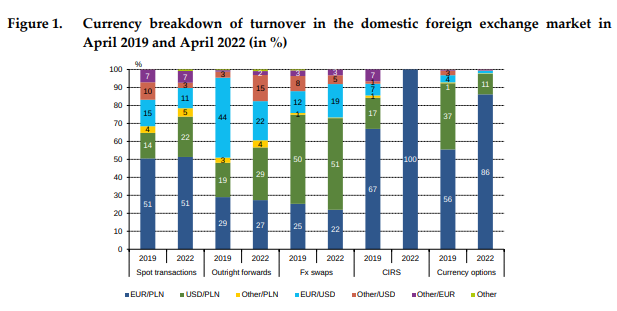
\includegraphics[width=0.85\textwidth]{plots/nbp_fx_poland_2022_breakdown.png}
  \caption{Struktura walutowa obrotu na krajowym rynku walutowym w Polsce w 2019 i 2022 roku (w \%). Źródło: NBP (2022), \textit{Wyniki badania rynku walutowego i rynku pozagiełdowych instrumentów pochodnych}.}
  \label{fig:nbp_breakdown}
\end{figure}

Z kolei struktura terminowa transakcji \textit{forward} i \textit{FX swap} wskazuje, że dominują operacje o krótkim horyzoncie – do siedmiu dni – które stanowią ponad 70\% wszystkich transakcji. 
Krótkoterminowy charakter obrotu potwierdza, że polski rynek walutowy służy przede wszystkim bieżącemu zarządzaniu płynnością i zabezpieczaniu pozycji, a nie długoterminowej spekulacji. 
Taka struktura jest typowa dla rynków rozwijających się, na których głównymi uczestnikami są banki komercyjne, instytucje finansowe i przedsiębiorstwa o ekspozycji na handel zagraniczny.

\begin{figure}[h!]
  \centering
  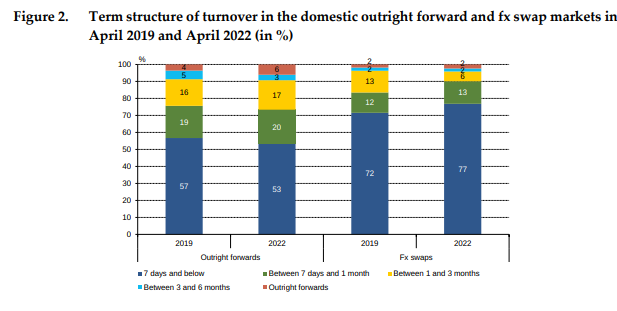
\includegraphics[width=0.8\textwidth]{plots/nbp_fx_poland_2022_swap.png}
  \caption{Struktura terminowa transakcji \textit{forward} i \textit{FX swap} na rynku krajowym w 2019 i 2022 roku (w \%). Źródło: NBP (2022).}
  \label{fig:nbp_swap_structure}
\end{figure}

Według danych Komisji Nadzoru Finansowego, w Polsce aktywnie inwestuje na rynku Forex około 80–100 tysięcy inwestorów detalicznych. 
Choć stanowią oni niewielki odsetek wszystkich uczestników rynku, ich rola stopniowo rośnie dzięki rozwojowi platform transakcyjnych i popularyzacji inwestowania online. 
Charakterystyczne jest jednak to, że większość obrotu generowana przez tę grupę ma charakter krótkoterminowy i spekulacyjny. 
Statystyki KNF wskazują, że około 70–80\% inwestorów detalicznych ponosi straty, co wynika przede wszystkim z wysokiego poziomu dźwigni finansowej oraz niedostatecznego zarządzania ryzykiem \parencite{knf2023}. 
Jednocześnie instytucje nadzorcze, w tym KNF i ESMA, prowadzą działania edukacyjne i regulacyjne, które mają na celu zwiększenie świadomości inwestorów i ograniczenie nadmiernego ryzyka w segmencie detalicznym.

Podsumowując, dane empiryczne BIS i NBP potwierdzają, że rynek walutowy, zarówno globalny, jak i krajowy, charakteryzuje się wysoką płynnością i dynamicznym wzrostem. 
W Polsce szczególnie istotną rolę odgrywają transakcje krótkoterminowe oraz operacje z udziałem złotego, które są ściśle związane z bieżącymi potrzebami finansowania handlu i zarządzania płynnością. 
Równocześnie rosnąca aktywność inwestorów indywidualnych, mimo wysokiego poziomu ryzyka, świadczy o zwiększającym się zainteresowaniu rynkiem Forex wśród uczestników detalicznych. 
Perspektywy dalszego rozwoju rynku w Polsce będą w dużej mierze zależeć od poziomu stabilności makroekonomicznej, 
regulacji europejskich oraz innowacji technologicznych wspierających dostęp do globalnych rynków finansowych.